\chapter{\IfLanguageName{dutch}{Stand van zaken}{State of the art}}%
\label{ch:stand-van-zaken}

% Tip: Begin elk hoofdstuk met een paragraaf inleiding die beschrijft hoe
% dit hoofdstuk past binnen het geheel van de bachelorproef. Geef in het
% bijzonder aan wat de link is met het vorige en volgende hoofdstuk.

% Pas na deze inleidende paragraaf komt de eerste sectiehoofding.

In dit hoofdstuk wordt de literatuurstudie besproken. 
Door deze literatuurstudie is het mogelijk om een beter inzicht te krijgen in de technologie en mogelijkheden voor de documentatie van Pythonprojecten alsook hoe het toegepast kan worden met behulp van Large Language Modellen. 
Er zal nadruk worden gelegd op bestaande literatuur en onderzoeken die verbonden zijn met documentatie van Pythonprojecten. 
In dit onderdeel zullen verschillende hoofdstukken worden aangekaart. 
Als eerste zal er duidelijk gemaakt worden wat er juist verstaan wordt onder documentatie. 
Vervolgens wordt er gekeken naar bestaande documentatie tools.
In het derde deel van deze literatuurstudie wordt er gekeken naar wat Large Language Modellen zijn, hoe deze werken en wat enkele bestaande modellen zijn.

\section{Wat is documentatie?}
\label{sec:wat-is-documentatie}

Alvorens er dieper op het onderwerp kan worden ingegaan, is het belangrijk dat er een duidelijk beeld gevormd wordt wat documentatie is. 
Waarom is documentatie belangrijk voor een project en wat wordt er begrepen onder documentatie? 

Documentatie is het proces van het vastleggen van de werking van een project.
Volgens \textcite{CodeQuality2024} kan dit op verschillende manieren gebeuren. 
Er kan gekozen worden om de documentatie te schrijven in de vorm van een commentaar in de code, een docstring, een API voor klassen of functies of in de vorm van een README.md bestand \autocite{CodeQuality2024}.
Het doel van documentatie is om de werking van het project te beschrijven zodat andere programmeurs het project kunnen begrijpen en gebruiken.
Zo gaat er geen tijd verloren aan het lezen van de code en het begrijpen ervan.

Documentatie kan gemaakt worden voor verschillende doelgroepen. Het kan voor interne of externe doeleinden zijn.
Interne documentatie is voor documentatie binnen hetzelfde bedrijf.
Dit gaat dan om het capteren van de proces kennis die vergaard is binnen een project. Dit is informatie zoals een roadmap of product requirements. 
Deze documentatie gaat over het vastleggen van gedetaïlleerde uitleg over hoe iets werkt en hoe het onderhouden kan worden \autocite{swimm.io2024}.

Externe documentatie is voor documentatie die gedeeld wordt met andere bedrijven of klanten. 
Dit gaat dan over de basiswerking van de code van een project zodat andere programmeurs het kunnen gebruiken.
Gebruiksaanwijzingen of handleidingen zijn ook een vorm van externe documentatie \autocite{swimm.io2024}.

Voor deze bachelorproef wordt er gekeken naar het documenteren van een Pythonproject in de vorm van commentaar in de code en het genereren van een samenvattend document van het gehele project.
Omdat Python een populaire programmeertaal is volgens \textcite{TIOBE2024} en er veel projecten in deze taal geschreven worden is het interessant om te kijken hoe deze projecten gedocumenteerd kunnen worden.
Ook kan er in de code bij functies aan type hinting gedaan worden. Dit indiceert wat de datatypes van de input en output van een functie zijn \autocite{Bailey2024}.
Uit deze documentatie kan de werking van het project duidelijk worden en kunnen de relaties tussen de verschillende bestanden en functies weergegeven worden.

In het verdere verloop van deze bachelorproef wordt er gekeken hoe de documentatie van een Pythonproject gegenereerd kan worden.

\subsection{Bestand documentatie}
\label{sec:bestand-documentatie}
Eerst dienen de bestanden van het project gedocumenteerd te worden.
Dit gebeurt door de code van het bestand te analyseren en de docstrings van de verschillende functies en klassen te genereren.

Docstrings of documentatie strings worden aan het begin van een functie of klasse geplaatst.
Deze strings worden gebruikt om de functie of klasse te documenteren \autocite{GeeksforGeeks2023}.
Volgens \textcite{GeeksforGeeks2023} zijn docstrings vitaal in het overdragen van het doel en de werking van een functie of klasse.

Deze docstrings kunnen dan gebruikt worden om een samenvatting van het bestand te genereren.

\subsection{Project documentatie}
\label{sec:project-documentatie-literatuur}
De documentatie van het project wordt gemaakt door de samenvattingen van de verschillende bestanden te combineren.
Deze samenvattingen worden gegenereerd op basis van de samenvatting van de bestanden die tot het project behoren.
In deze samenvatting behoort de werking van het project, de verschillende bestanden met functies en klassen en de relaties tussen deze bestanden.


\section{Bestaande documentatie tools}
\label{sec:huidige-tools}
Voor er gekeken wordt hoe LLM's mogelijk gebruikt kunnen worden voor het genereren van documentatie is het belangrijk dat er een helder beeld is van de huidige tools die gebruikt worden voor het genereren van documentatie.
De documentatie kan in verschillende vormen gegeneerd worden. Dit kan gaan van een website tot een samenvattend document.
Ook kunnen er in de code zelf commentaren geplaatst worden die de werking van de code uitleggen.
Hiervoor bestaan er reeds verschillende tools en dit voor verschillende programmeertalen opgelijst in tabel \ref{table:vgl-tools}.
In dit onderdeel is er enkel gekeken naar tools die nog onderhouden worden door de makers. 

\subsection{Doxygen}
Doxygen \autocite{Doxygen2023} is een tool die het toelaat om automatisch code documentatie te genereren. Het is een gratis tool die bruikbaar is voor verschillende programmeertalen zoals: C++, C, Python, PHP en Java.
Het genereert documentatie in de vorm van HTML, LaTeX, RT. 
Deze tool is in staat om een diagram te genereren met de relaties tussen de verschillende delen van de code bijvoorbeeld de relaties tussen de verschillende klassen en functies.
Een voorbeeld van een diagram kan gezien worden in figuur \ref{fig:Doxygen-diagram}.
Zo wordt er een duidelijk beeld verkregen van de structuur van het project.

\begin{figure}[h]
  \centering
  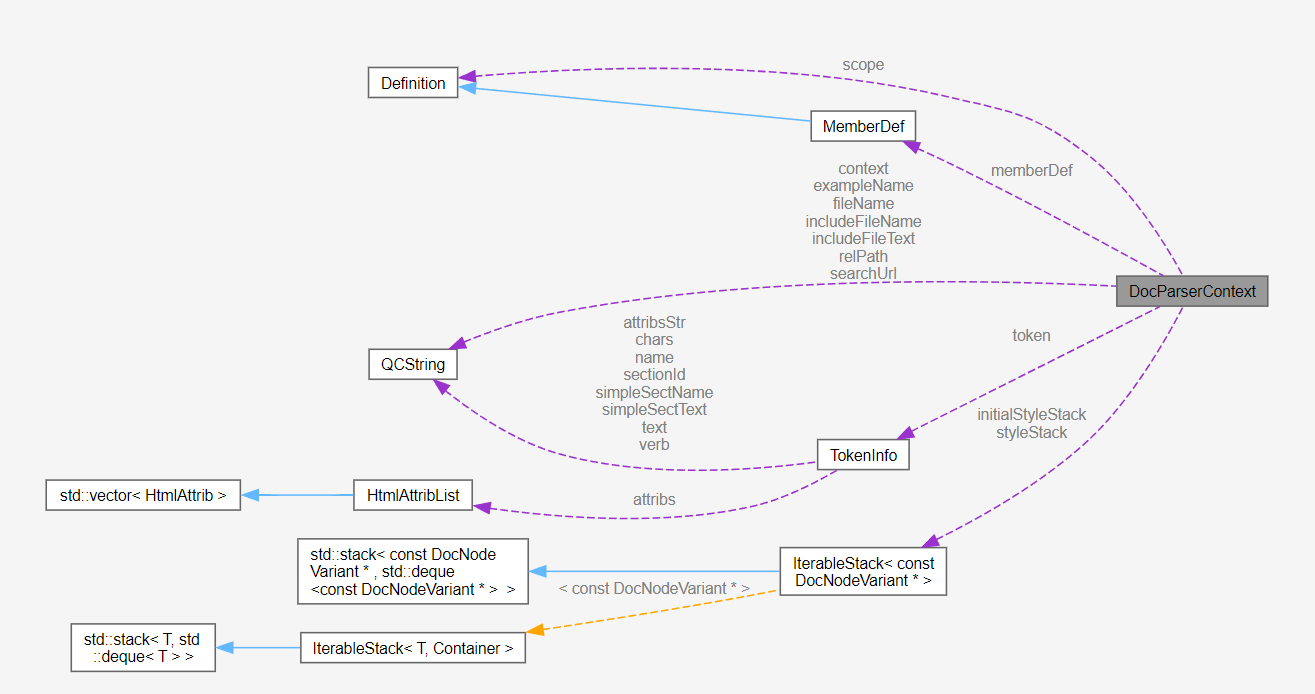
\includegraphics[width=1\textwidth]{doxygen_diagram.png}
  \caption{Voorbeeld diagram van Doxygen \autocite{Doxygen2023}}
  \label{fig:Doxygen-diagram}
\end{figure}

\subsection{CodeCat}
\textcite{CodeCat2024} is een online tool die de code analyseert en de docstrings genereert. Er kan niet gekeken worden naar de werking van CodeCat aangezien het niet open sourced is.
Deze tool genereert automtisch de docstrings voor JavaScript code.

\subsection{GPT4Docstrings}
De tool van \textcite{Trofficus2023} genereert docstrings voor Python code. Het maakt gebruik van GPT-4 \autocite{OpenAI2023} om de docstrings te genereren.
Deze tool leunt sterk aan bij de doelstelling van deze bachelorproef, namelijk het genereren van documentatie met behulp van LLM's.
Het nader bekijken van deze tool kan een meerwaarde zijn voor deze bachelorproef.

\begin{figure}
  \centering
  \begin{subfigure}[b]{0.5\textwidth}
      \centering
      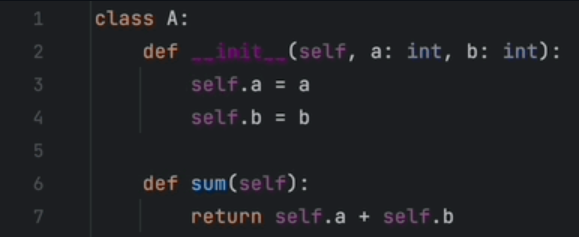
\includegraphics[width=1\textwidth]{before_troficus.png}
      \caption{Voorbeeld code zonder docstrings van \textcite{Trofficus2023}}
      \label{fig:before-Trofficus}
  \end{subfigure}
  \hfill
  \begin{subfigure}[b]{0.5\textwidth}
      \centering
      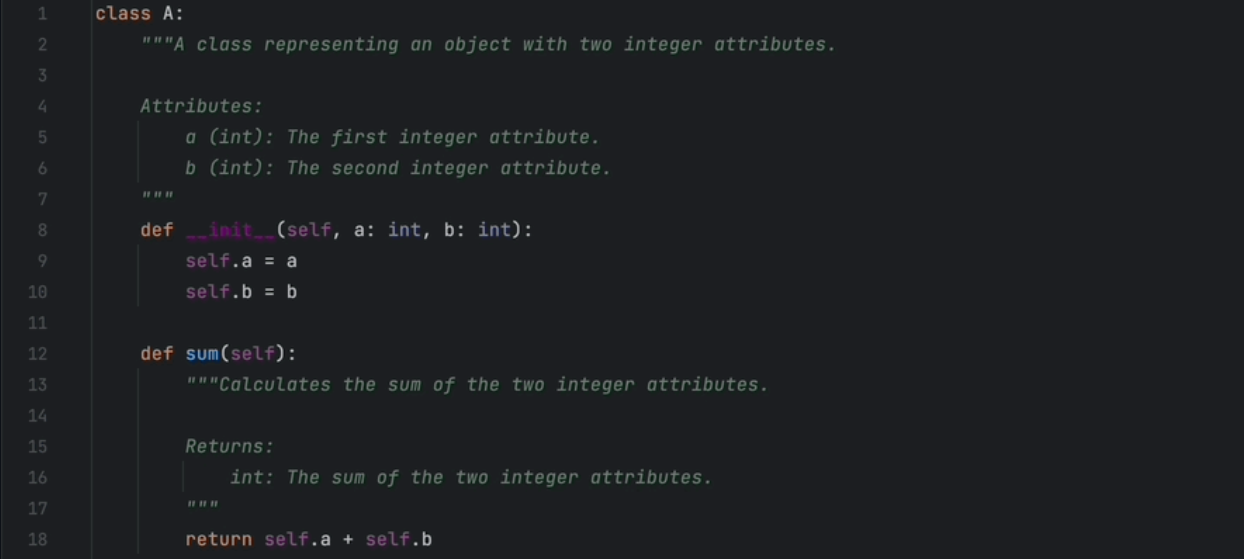
\includegraphics[width=1\textwidth]{after_troficus.png}
      \caption{Voorbeeld code met docstrings van \textcite{Trofficus2023}}
      \label{fig:after-Trofficus}
  \end{subfigure}
     \caption[Uitkomst GPT4Docstrings]{Voorbeeld uitkomst van de tool van \textcite{Trofficus2023}}
     \label{fig:Before-After-Trofficus}
\end{figure}

Zo gebruikt GPT4Docstrings van \textcite{Trofficus2023} de Abstract Syntax Tree (AST) van de code om de structuur van de code te begrijpen.
Uit de AST kunnen de juiste stukken code gehaald worden om de docstrings te genereren.
Dit kan goed van pas komen voor het genereren van documentatie van Pythonprojecten.
Een voorbeeld van deze tool kan gezien worden in figuur \ref{fig:Before-After-Trofficus}. 

\subsection{Sphinx}
Sphinx van \textcite{Sphinx2023} is één van de meest gebruikte tools voor het genereren van documentatie voor Pythonprojecten.
Het genereert documentatie aan de hand van docstrings. Het toont de hiërarchie van het project om een duidelijk overzicht te geven.
Deze tool is vrij flexibel want het kan uitgebreid worden met verschillende extensies, zodat het alle mogelijke wensen kan vervullen.
Volgens \textcite{Sphinx2023} kan de extensie autodoc semi-automatisch de docstrings van een module extraheren en in de documentatie plaatsen. 
Handig wanneer de automatische documentatie generatie van een geheel project gewenst is. Zo kan het project samengevat worden aan de hand van de docstrings van de verschillende python files. 
Alvorens een Python project gedocumenteerd kan worden met Sphinx \autocite{Sphinx2023}, dienen alle bestanden aangevuld te worden met docstrings.
Dit gebeurt echter niet bij het runnen van het programma.

\subsection{Pdoc}
Pdoc \autocite{GallantHils2023} genereert documentatie in de vorm van een website die een API van de documentatie bevat. 
Hier kan er eenvoudig op de website gezocht worden naar een functie of klasse met de bijhorende documentatie.

\begin{table}[h!]
\centering
\resizebox{\textwidth}{!}{
\begin{tabular}{|c|c|c|}
\hline
Tool & programmeertaal & type \\ [0.5ex]
\hline
Doxygen & C++, C, Python, PHP, Java & HTML, PDF, markdown\\
\hline
CodeCat & JavaScript & docstring \\
\hline
Sphinx & Python & HTML, LATEX, man pages \\
\hline
Pdoc & Python & API \\
\hline
GPT4Docstrings & Python & docstring \\
\hline
\end{tabular}}
\caption{Vergelijking documentatie tools}
\label{table:vgl-tools}
\end{table}

\subsection{Samenvatting tools}
\label{sec:samenvatting-tools}
Door de verschillende tools op te lijsten en te vergelijken met elkaar wordt er een duidelijk beeld gevormd van wat de tools kunnen genereren.
Zo kan er een keuze gemaakt worden welke tool het beste past bij dit onderzoek.
In tabel \ref{table:ra-tools} wordt er een overzicht gegeven wat de tools kunnen genereren.
De tools Doxygen, Sphinx en Pdoc kunnen enkel een document genereren in de vorm van een website of een bestand op basis van reeds bestaande docstrings en commentaren in de code.
De tool GPT4Docstrings genereert docstrings voor Python code met behulp van een LLM.

\begin{table}[h!]
  \centering
  \resizebox{\textwidth}{!}{
  \begin{tabular}{|c|c|c|c|c|}
  \hline
  Tool & docstrings & samenvatting bestand & samenvatting project & visualisatie \\ [0.5ex]
  \hline
  GPT4Docstrings & ja & nee & nee & nee \\
  \hline
  Doxygen & nee & nee & nee & ja \\
  \hline
  Sphinx & nee & nee & nee & nee \\
  \hline
  Pdoc & nee & nee & nee & nee \\
  \hline
  \end{tabular}}
  \caption{Overzicht van wat de tools kunnen genereren}
  \label{table:ra-tools}
  \end{table}

\section{Wat zijn Large Language Modellen (LLM)?}
\label{sec:wat-zijn-llms}

Uit de vorige sectie is gebleken dat er slechts één tool geschikt is voor het genereren van documentatie voor projecten zonder gedocumenteerde code. 
De tool GPT4Docstrings van \textcite{Trofficus2023} maakt gebruik van een Large Language Model (LLM) om de docstrings te genereren.
Het is dus belangrijk dat er een duidelijk beeld is van wat LLM's juist zijn en hoe deze werken.
Wat kunnen deze modellen, wat zijn de mogelijke beperkingen en wat is de huidige stand van zaken. 
In dit hoofdstuk wordt er een antwoord gegeven op de vragen: 
\begin{itemize}
  \item Bestaan er LLM's speciaal getraind op Python code? 
  \item Kunnen LLM's gebruikt worden om documentatie te genereren?
\end{itemize}

Dit draagt bij tot het verkrijgen van een grondige basiskennis van LLM's. 
Het veld waarin AI zich bevind wordt vaak voorgesteld volgens figuur \ref{fig:LLM-position}, met verschillende lagen \autocite{Stoeffelbauer2023}.
Deze lagen zijn: Artificiële Intelligentie, Machine Learning, Deep Learning en Large Language Modellen.
Omdat LLM's een subveld zijn van Deep Learning is het belangrijk dat er een duidelijk beeld is van wat Deep Learning juist is.
Uit de figuur \ref{fig:LLM-position} blijkt dat AI verschillende categorieën omvat.
AI is een brede term vermeldt \textcite{Stoeffelbauer2023} hiermee wordt vaak verwezen naar slimme machines. 
Machine Learning (ML) is een subveld van AI, waarin patronen worden herkend tussen een input en een output.
ML kan gebruikt worden voor verschillende taken zoals classificatie, regressie, clustering en dergelijke.
Volgens \textcite{Stoeffelbauer2023} is Deep Learning (DL) een subveld van ML, waarin complexe algoritmen en Deep Neural Networks gebruikt worden om complexere taken uit te voeren.
Deep Learning is een krachtige tool die gebruikt wordt voor verschillende taken zoals: beeldherkenning, spraakherkenning, ...

\begin{figure}[h]
  \centering
  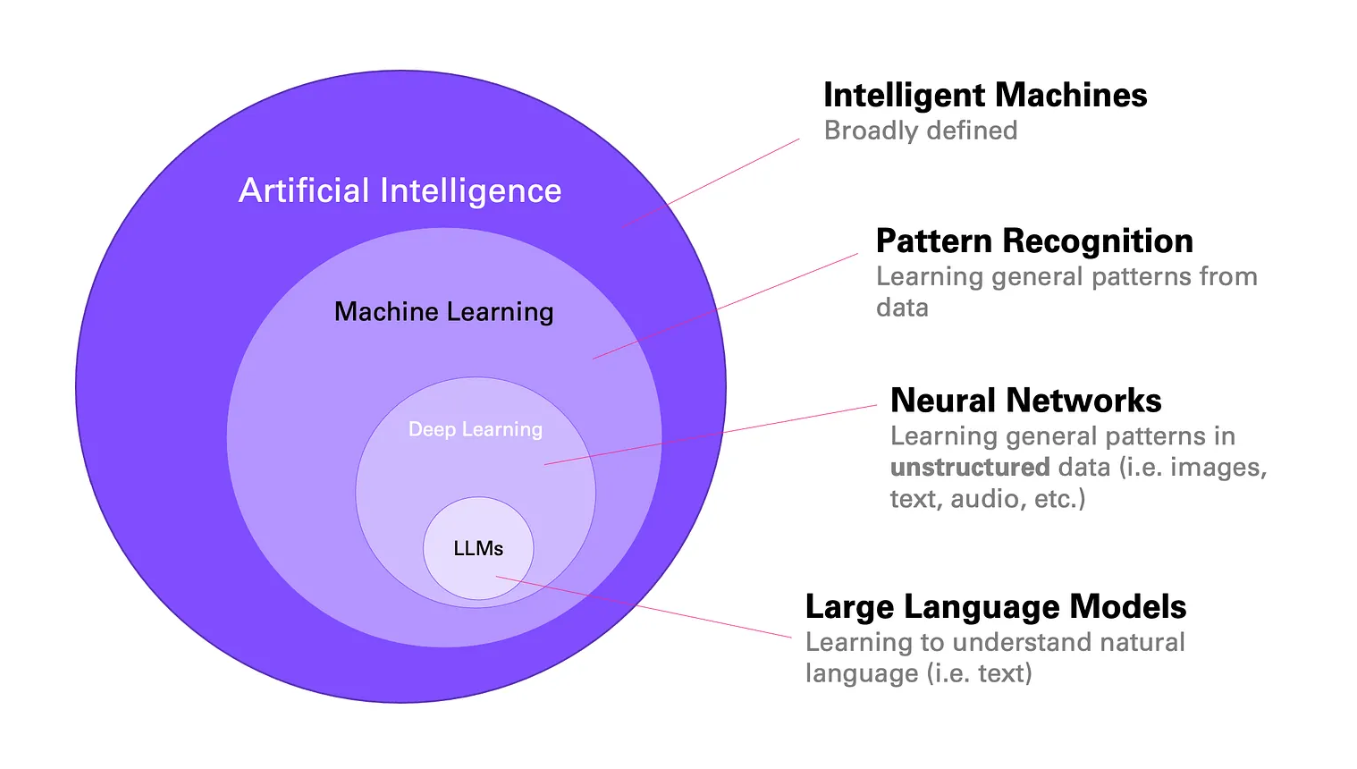
\includegraphics[width=0.5\textwidth]{LLMsphere.png}
  \caption{Artificiële intelligentie in lagen \autocite{Stoeffelbauer2023}}
  \label{fig:LLM-position}
\end{figure}

Large Language Modellen zijn geavanceerde AI-systemen die dienen om menselijke taal te verstaan, te genereren en te verwerken.
LLM's worden getraind op een grote hoeveelheid tekst wat vaak uit allerlei data zoals artikels of websites gehaald wordt. 
Volgens \textcite{Beelen2023} zorgen Deep Neural Networks ervoor dat LLM's natuurlijke taal verwerken op een gelijkaardige manier die vergelijkbaar is met de menselijke taalvaardigheid.
Deze hebben een grote vooruitgang gekend in 2017 door de paper van \textcite{VaswaniEtAl2017}. 
Hieruit kwam een nieuw mechanisme tot stand namelijk transformers wat bestaat uit Attentie blokken. 
Enkele voordelen die komen kijken bij het gebruiken van transformers zijn: 
\begin{itemize}
  \item Het kan lange sequenties verwerken.
  \item Het kan parallel sequenties verwerken.
  \item Het kan de relaties tussen de verschillende delen van de sequentie leren.
\end{itemize}
Hierdoor hebben transformer modellen een snellere trainingsperiode dan vorige neurale netwerken \autocite{aiml2023}.

\subsection{Transformers en de architectuur van LLM's}
\label{sec:architectuur-van-llms}
Omdat in dit onderzoek gebruik gemaakt wordt van LLM's is het nodig dat er dieper ingegaan wordt op de architectuur van deze modellen om een beter inzicht te krijgen hoe deze werken.
Een neuraal netwerk bestaat uit verschillende lagen. Enkele belangrijke blokken die gebruikt worden binnen de transformer laag zijn:
\begin{itemize}
  \item Self-Attention
  \item Cross-Attention
  \item Masked Self-Attention
\end{itemize}

Deze Attentie blokken worden gebruikt in de encoder en decoder van een transformer en stromen voort uit het onderzoek van \textcite{VaswaniEtAl2017}.

Transformers zijn een speciaal type van neurale netwerken die gebruik maken van verschillende Attentie blokken.
Attentie is een mechanisme dat gebruikt wordt om de relaties tussen verschillende delen van de invoersequenties te leren.
Een transformer bestaat uit een encoder en een decoder. 
Niet elke transformer bestaat uit zowel een encoder als een decoder het kan ook enkel encoder of decoder bevatten \autocite{Hoque2023}.
De encoder wordt gebruikt om de invoersequenties te verwerken en de decoder wordt gebruikt om de uitvoersequenties te genereren.
Zo is BERT van \textcite{DevlinEtAl2019} een transformer die enkel een encoder heeft en GPT van \textcite{RandfordEtAL2018} heeft enkel een decoder.
De transformer architectuur uit de paper van \textcite{VaswaniEtAl2017} kan gezien worden in figuur \ref{fig:transformer-model}. 

Self-Attention duidt dynamische gewichten toe aan verschillende elementen binnen de meegegeven sequentie, bijvoorbeeld woorden in een zin.
Dit laat het model toe om zich te concentreren op de meest relevante delen van de invoer, terwijl de invloed van minder cruciale delen wordt verminderd.
De invoersequentie wordt eerst in drie verschillende vectoren omgezet: Query, Key en Value.
De Query vector stelt een specifiek token uit de invoersequentie voor. De Key vector vertegenwoordigt alle tokens en de vector voor Value bevat de feitelijke inhoud die aan elk token is gekoppeld.
De similariteit tussen de Query en de Key vector wordt berekend aan de hand van het inwendig product van de twee vectoren.
Deze similariteit wordt gebruikt om de gewichten te berekenen die aan de Value vector worden toegekend \autocite{VaswaniEtAl2017}.

Masked Self-Attention is een variant van Self-Attention die gebruikt wordt in de decoder van een transformer.
In de decoder wordt er een mask gebruikt om enkel de vorige tokens te zien in de sequentie \autocite{VaswaniEtAl2017}.
Dit vermijdt dat er informatie van de toekomstige tokens gebruikt wordt. 
Zo kan de transformer niet "vals spelen" tijdens het train proces.

Cross-Attention is een variant van Self-Attention die gebruikt wordt in de decoder van een transformer.
Deze laag gebruikt de informatie van de encoder en de vorige Attentie laag van de decoder om de uitvoersequenties te genereren.
De Query vector is de uitvoer van de vorige Attentie/Cross-Attention laag van de decoder en de Key en Value vector zijn de uitvoer van de encoder \autocite{VaswaniEtAl2017}.
Doordat de Cross-Attentione laag informatie van zowel de encoder als decoder krijgt kan het model de relaties tussen de verschillende delen van de invoersequenties leren.
Deze relaties worden dan gebruikt om de uitvoersequenties te genereren.

\begin{figure}[h]
  \centering
  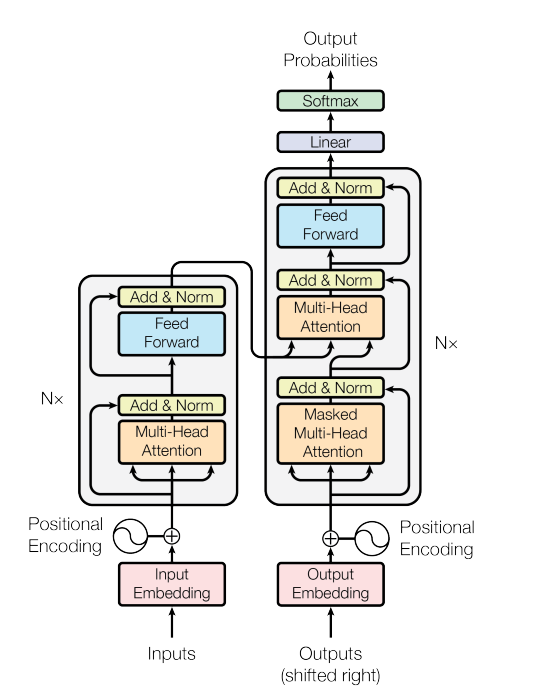
\includegraphics[width=0.5\textwidth]{transformer.png}
  \caption[Architectuur transformer model]{Transformer model architectuur \autocite{VaswaniEtAl2017}}
  \label{fig:transformer-model}
\end{figure}

\subsection{Trainen van LLM's}
\label{sec:trainen-van-llms}
Het trainen van LLM's is een complex proces dat veel tijd en rekenkracht vereist. Dit gebeurt in verschillende stappen.
De eerste fase begint bij het verzamelen van een grote hoeveelheid tekst die gebruikt wordt om het model te trainen.
Deze tekst wordt gehaald uit verschillende artikelen, websites, boeken en andere bronnen. 

Zo kan het volgende woord in een sequentie van tekst voorspeld worden.

Het model krijgt deze grote hoeveelheid tekst in de pre-training fase.
In deze fase leert de LLM grammatica, semantiek, taal patronen en factuele informatie \autocite{Cacic2023}.
Voordat de data meegegeven wordt aan het model moet de data gecleaned en geformatteerd worden.
Dit gebeurt in het tokenization proces. 
Hier wordt de tekst omgezet in tokens die het model kan verwerken \ref{fig:tokenization}.
Woorden kunnen kleiner gemaakt worden zodat de volledige tekst in het model past. 
Dit gebeurt wanneer het model een beperkte input capaciteit heeft \autocite{ElHousieny2023}.
Deze woorden worden dan omgezet wordt in embeddings en deze embeddings worden meegegeven aan het model om het te trainen.
Uit de data kunnen dan patronen gehaald worden met behulp van Transformers \ref{sec:architectuur-van-llms}, maar het is nog niet in staat om vragen of instructies te begrijpen.

\begin{figure}[h]
  \centering
  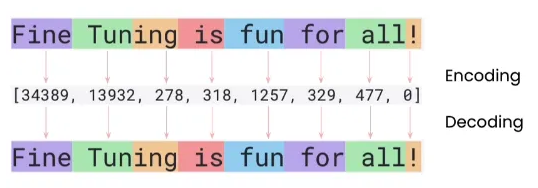
\includegraphics[width=0.5\textwidth]{tokenization.png}
  \caption[Tokenisatie van tekst]{Gesimplificeerde tokenisatie van tekst \autocite{TeeTracker2023}}
  \label{fig:tokenization}
\end{figure}

De volgende fase bestaat uit het trainen van het model op een dataset met instructies en het antwoord erop. 
Volgens \textcite{Das2024} is dit het gesuperviseerde Fine-Tunen van een LLM.
In deze fase probeert het model de patronen te leren die nodig zijn om vragen te beantwoorden of instructies te volgen.
Dit zorgt ervoor dat het model instructies kan volgen en vragen leert te beantwoorden.

Er kan gebruik gemaakt worden om het model specifiek aan de wensen van de mens te laten voldoen. Dit kan door het gebruiken van Reinfocement Learning met menselijke feedback \autocite{LambertEtAL2022}. 
Hierbij geeft de mens feedback aan het model en leert het model bij door deze feedback.

\subsection{Fine-Tuning van LLM's}
\label{sec:fine-tuning-van-llms}

Volgens \textcite{Peckham2024} kan het model achteraf nog extra getraind worden op een specifieke dataset zoals Python code of medische data.
Dit proces heet het Fine-Tunen van een LLM.
Enkele vereisten voor het Fine-Tunen van een LLM zijn de dataset moet een grote hoeveelheid data hebben.
Ook moet de dataset van hoge kwaliteit zijn en moet de dataset het onderwerp representatief voorstellen \autocite{Peckham2024}.

\subsection{Prompt Engineering}
\label{sec:prompt-engineering}

Prompt Engineering is een techniek die gebruikt wordt om de uitkomst van een LLM te beïnvloeden volgens \textcite{Google2023}.
Er wordt een prompt gegeven aan het model met duidelijke instructies over wat er verwacht wordt. 
Wanneer deze instructies niet voldoen, wordt de prompt iteratief aangepast en wordt de uitkomst geëvalueerd totdat de gewenste uitkomst is bereikt.
Dit iteratieve proces heet Prompt Engineering \autocite{Trad2024}.

Door het toevoegen van enkele voorbeelden aan de prompt kan het model beter begrijpen wat er verwacht wordt \autocite{OpenAi2024a}.
\begin{itemize}
  \item Geef structuur aan de prompt.
  \item Geef een rol mee.
  \item Geef een context.
  \item Geef een doel.
\end{itemize} 
Dit zijn de beste manieren om een prompt te structureren volgens \autocite{Google2023}.

\subsection{Bestaande LLM's}
\label{sec:bestaande-llms}

Momenteel zijn er verschillende LLM's die gebruikt worden voor verschillende taken.
Deze LLM's zijn getraind op verschillende datasets en hebben verschillende architecturen.
Het is belangrijk dat er een duidelijk beeld is van de verschillende LLM's en hun mogelijkheden. 
Met dit beeld kan er een goede keuze gemaakt worden voor het genereren van documentatie.

Eén van de grote spelers in de wereld van LLM's is OpenAI. OpenAI heeft verschillende LLM's ontwikkeld gaande van GPT \autocite{RandfordEtAL2018} tot GPT-4 \autocite{OpenAI2023}.
Het is getraind op een grote hoeveelheid data en heeft een grote capaciteit.
Een nadeel is dat GPT-4 een betalende service is \autocite{OpenAI2023}.

Een andere grote speler is Google. Google heeft verschillende LLM's ontwikkeld waaronder BERT van \textcite{DevlinEtAl2019} en Gemini \autocite{Google2024}.
BERT staat voor Bidirectional Encoder Representations from Transformers, een DL model waar elk output element verbonden is met elk input element \autocite{HashemiPour2024}.
BERT was een eerste stap in de wereld van LLM's voor Google. Sinds kort heeft \textcite{Google2024} een nieuwe LLM ontwikkeld genaamd Gemini.
Deze LLM is een sterke concurrent voor GPT-4 van \textcite{OpenAI2023}. 

Google \autocite{Google2024} bracht een model met verschillende versies uit: Gemini Pro, Gemini Ultra en Gemini Nano. 
Elke versie is gemaakt voor een specifiek doel. Zo is Gemini Nano het meest efficiënte model voor mobiele toestellen, terwijl Gemini Pro het beste model is voor het schalen van allerlei taken.
En Gemini Ultra is het meest capabele en grootste model van Google, dit kan gebruikt worden voor complexe taken.
Een van de voordelen van Gemini is dat er een groot aantal input tokens meegegeven kunnen worden, namelijk 1 miljoen tokens \autocite{Google2024}.
Dit is aanzienlijk meer dan de 128 duizend tokens van GPT-4.

Een derde speler in de wereld van LLM's is Meta. Meta heeft verschillende LLM's ontwikkeld onder de naam LLama 2 \autocite{Meta2024}.
De LLama 2 familie bestaat uit verschillende LLM's die getraind zijn op verschillende data. Sommige zijn extra getraind voor specifiekere doeleinden.
Zo is er bijvoorbeeld een LLM getraind op Python code, genaamd Code LLama 2 van \textcite{Roziere2024}.
Een voordeel van de LLama 2 familie is dat deze LLM's open source zijn en dus voor iedereen toegankelijk zijn.

Antropic heeft ook een LLM ontwikkeld genaamd Claude \autocite{Anthropic2023}. 
Claude's capaciteiten zijn code generatie, het verstaan van meerdere talen, beelden analyseren en kan geavanceerde redeneringen geven.
Er bestaan 3 versies van Claude: Haiku, Sonnet en Opus.
Haiku is een lichte versie van Claude en Sonnet is de combinatie van performantie en snelheid. Opus is het intelligentste model dat complexe taken kan uitvoeren en begrijpen.
Claude is een betalende service en de prijzen zijn afhankelijk van de gekozen versie van Claude \autocite{Anthropic2023}.

De verschillen tussen deze LLM's zijn groot, zo is er een verschil in capaciteit, trainingsdata en toegankelijkheid.
Het is belangrijk dat er een goede keuze gemaakt wordt voor het genereren van documentatie.
Deze keuze zal afhangen van de mogelijkheden van de LLM's en de doeleinden van de documentatie.

\begin{table}[h!]
\centering
\resizebox{\textwidth}{!}{
\begin{tabular}{|c|c|c|c|c|} 
  \hline
  Model & Input (1M tokens) & Output (1M tokens) & Context & Snelheid (t/s)\\ [0.5ex] 
  \hline
  GPT-4 Turbo \autocite{OpenAi2024} & \$10.00 & \$30.00 &  128k & 18\\ 
  \hline
  GPT-4 \autocite{OpenAi2024} & \$30.00 & \$60.00 &  128k & 21\\ 
  \hline
  GPT-3.5 Turbo \autocite{OpenAi2024} & \$0.50 & \$1.50 &  16k & 52\\
  \hline
  Gemini 1.5 Pro \textcite{Google2024} & \$3.50 & \$10.50 &  128k & 52\\
  \hline
  Code LLama \autocite{Meta2024} & \$0.90 & \$0.90 & 100k & 34\\
  \hline
  LLama 2 \autocite{Meta2024} & \$0.95 & \$1.00 & 100k & 34\\
  \hline
  Claude Opus \autocite{Anthropic2023} & \$15.00  & \$75 &  200k & 29\\
  \hline
  Claude Sonnet \autocite{Anthropic2023} & \$3.00  & \$15 &  200k & 61\\ 
  \hline
  Claude Haiku \autocite{Anthropic2023} & \$0.20  & \$1.20 &  200k & 102\\
  \hline
\end{tabular}}
\caption{Vergelijking van verschillende LLM's op basis van prijs (\$), context (aantal tokens) en snelheid (Tokens per seconde) \autocite{ArtificialAnalysis2024}}
\label{table:vgl-llms}
\end{table}

In de tabel \ref{table:vgl-llms} wordt een vergelijking gemaakt tussen verschillende LLM's.
Hierin wordt er gekeken naar de prijs van de input en output tokens, de grootte van de context en het aantal tokens dat per seconde verwerkt kan worden.

\begin{table}[h!]
\centering
\resizebox{\textwidth}{!}{
\begin{tabular}{|c|c|c|c|}
\hline
Model & Coding & Beredenering en Kennis\\
\hline
GPT-4 Turbo \autocite{OpenAi2024} & 86\% & 85.4\% \\
\hline
GPT-4 \autocite{OpenAi2024} & 86\% & 88.4\% \\
\hline
GPT-3.5 Turbo \autocite{OpenAi2024} & 70\% & 73.2\% \\
\hline
Gemini 1.5 Pro \textcite{Google2024} & 82\% & 71.9\% \\
\hline
Code LLama \autocite{Meta2024} & /  & 67.8\% \\
\hline
LLama 2 \autocite{Meta2024} & 69\%  & / \\
\hline
Claude Opus \autocite{Anthropic2023} & 87\%  & / \\
\hline
Claude Sonnet \autocite{Anthropic2023} & 79\%  & / \\
\hline
Claude Haiku \autocite{Anthropic2023} & 75\%  & / \\
\hline
\end{tabular}}
\caption{Vergelijking LLM's op basis van beoordeling van menselijke evaluatie en MMLU \autocite{ArtificialAnalysis2024}}
\label{table:vgl-llms-eval}
\end{table}

In de tabel \ref{table:vgl-llms-eval} wordt een vergelijking gemaakt tussen verschillende LLM's tussen twee kolommen. 
De eerste kolom bevat de beoordeling van de coding mogelijkheden van het model gequoteerd met menselijke evaluatie. 
In de tweede kolom staat de quotering op basis van de MMLU een dataset \autocite{Hendrycks2020}.
Beide kolommen staan uitgedrukt in procenten met 100\% als maximum.
Hieruit kan geconcludeerd worden dat GPT-4 en GPT-4 Turbo de beste scores behalen op beide vlakken.
Maar omdat er in dit onderzoek gezocht wordt naar een goedkope oplossing wordt er geconcludeerd uit beide tabellen dat GPT-3.5 Turbo de beste prijs/kwaliteit verhouding heeft.
